\documentclass[aspectratio=169, 14pt]{beamer}
\usepackage[utf8]{inputenc}
\usepackage{xeCJK}
\usepackage{tipa}
\usepackage{graphicx}
\usepackage{transparent}
\usepackage[ruled, lined, linesnumbered, commentsnumbered]{algorithm2e}
\usepackage{tikz}
\usetikzlibrary{matrix,backgrounds}
\usetikzlibrary{arrows}
\usetikzlibrary {arrows.meta}
\usetikzlibrary{calc,shadows.blur,fit,positioning}
\usepackage{pgfplots} 
\usepackage{minted}
\usepackage{fontawesome5}
\usepackage{booktabs}
\usepackage{caption}
\usepackage{hyperref}
\hypersetup{
    colorlinks=true,
    linkcolor=blue,
    filecolor=magenta,      
    urlcolor=cyan,
    }
\urlstyle{same}
\usetheme{metropolis}
\metroset{block=fill}
\usecolortheme{default}
\definecolor{darkmidnightblue}{rgb}{0.0, 0.2, 0.4}
\definecolor{LightGray}{gray}{0.9}


%------------------------------------------------------------
%This block of code defines the information to appear in the
%Title page
\title[Database Principles and Applications] %optional
{数据库原理与应用}

\subtitle{Introduction to SQL}

\author[CHEN Zhongpu] % (optional)
{CHEN Zhongpu}

\institute[] % (optional)
{
  School of Computing and Artificial Intelligence \\
  \href{mailto:zpchen@swufe.edu.cn}{zpchen@swufe.edu.cn}
}

\date[] % (optional)
{SWUFE, Spring \the\year{}}

%End of title page configuration block
%------------------------------------------------------------


%------------------------------------------------------------
%The next block of commands puts the table of contents at the 
%beginning of each section and highlights the current section:

% \AtBeginSection[]
% {
%   \begin{frame}
%     \frametitle{Table of Contents}
%     \tableofcontents[currentsection]
%   \end{frame}
% }
%------------------------------------------------------------


\begin{document}

%The next statement creates the title page.
\frame{\titlepage}

%---------------------------------------------------------
%This block of code is for the table of contents after
%the title page
% \begin{frame}
% \frametitle{Table of Contents}
% \tableofcontents
% \end{frame}
%--------------------------------------------------------
\begin{frame}[fragile]
	\frametitle{复习}
	\begin{columns}
		\column{.35\textwidth}<1->
		\begin{itemize}
			\item 数据库、DBMS
			\item 关系模型
			\item DDL、DML
			\item 关系代数
		\end{itemize}
		\column{.64\textwidth}<2->
		Relation is essentially a mathematical term for table. Each table is a named collection of rows. Each row of a given table has the same set of named columns, and each column is of a specific data type. Whereas columns have a fixed order in each row, it is important to remember that DB does not guarantee the order of the rows within the table in any way.
	\end{columns}

\end{frame}

\begin{frame}[fragile]
	\frametitle{数据库查询语言:SQL}
	\begin{center}
		\begin{tikzpicture}[slot/.style={draw, minimum size=1.2cm,rectangle, rounded corners=0.1cm}]
			\matrix[nodes=draw, column sep=.5cm](first) {
				\node[slot, fill=blue!30]{DML}; & \node[slot, fill=blue!30]{DDL}; & \node[slot]{视图 (view)}; \\
			};
			\matrix[nodes=draw, column sep=.5cm, below=of first, yshift=1cm](second) {
				\node[slot]{完整性 (integrity)}; & \node[slot]{事务 (transaction)}; \\
			};
			\node[slot, below=of second, yshift=.8cm](third){授权(authorization)};
			\node[slot, below=of third, text width=10cm, yshift=.6cm](fourth){嵌入式、动态 SQL
				(embedded, dynamic SQL)
			};
		\end{tikzpicture}
	\end{center}


\end{frame}

{
% \usebackgroundtemplate{\transparent{0.3}{\begin{picture}
%     
\includegraphics[height=0.7\paperheight]{cover}
% \end{picture}    
% }}
\usebackgroundtemplate{
	\tikz[overlay,remember picture]
	\node[opacity=0.3, at=(current page.south east),anchor=south east, yshift=2cm,xshift=4cm] {
		
\includegraphics[height=0.6\paperheight]{cover}};
}
\begin{frame}
	\section{\textcolor{darkmidnightblue}{1. SQL}}
	Structured Query Language.

	\begin{itemize}
		\item \textipa{/""Es""kju:"El/}
		\item \textipa{/"si:kw@l/}
	\end{itemize}
	\bigskip
	\begin{quote}
		SQL is a domain-specific language used in programming and designed for managing data held in a RDBMS.
	\end{quote}
\end{frame}
}

\begin{frame}[fragile]
	\frametitle{1.1 SQL 的历史}
	\begin{tikzpicture}
		\node[inner sep=0pt] (ibm) {
			{
\includegraphics[width=.25\textwidth]{week3/ibm}}
		};
		\node[below=of ibm]{20世纪70时代,\textcolor{red}{Sequel}};

		\node[inner sep=0pt, right=of ibm, xshift=1.5cm] (anis) {
			{
\includegraphics[width=.25\textwidth]{week3/anis}}
		};
		\node[inner sep=0pt, right=of anis, xshift=-1.2cm] (iso) {
			{
\includegraphics[width=.25\textwidth]{week3/iso}}
		};
		\node[below=of anis, xshift=1.2cm]{1986 年
			,\textcolor{red}{SQL}};
	\end{tikzpicture}

	\textbf{SQL 语言一直在不断发展:}
	SQL-86、SQL-89、SQL-92、SQL: 1999、SQL: 2003、SQL: 2006、SQL: 2008、SQL: 2011、SQL: 2016、SQL: 2023
\end{frame}

\begin{frame}

	\begin{columns}
		\column{.475\textwidth}
		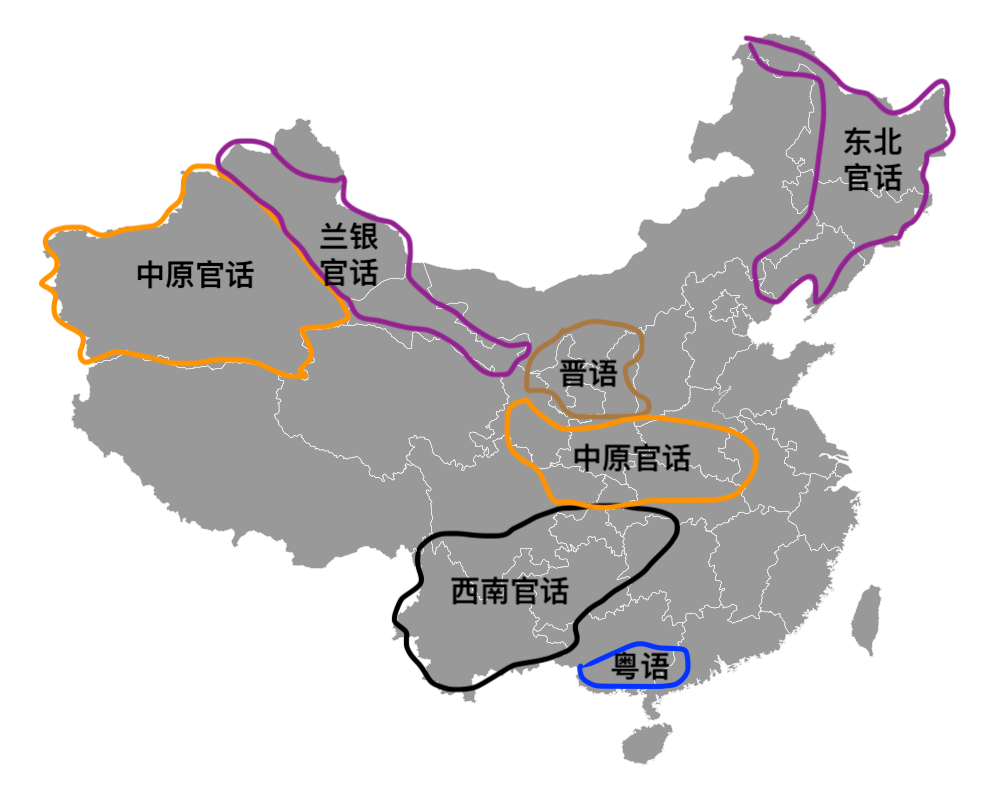
\includegraphics[width=\textwidth]{week3/china}
		\column{.475\textwidth}
		\begin{block}{SQL 方言}
			各家数据库产商并没有 100\% 实现标准 SQL,而是实现了大部分并加入了自己的扩展,被称为 \alert{SQL 方言} (dialect)。
		\end{block}
	\end{columns}

	虽然有「标准的」SQL,但实际使用的都是「不标准的」SQL。

	\begin{itemize}
		\item PostgreSQL
		\item MySQL
		\item SQLServer
		\item ...
	\end{itemize}
\end{frame}

\begin{frame}[fragile]
	\frametitle{1.2 SQL 的流行程度}
	\begin{figure}
		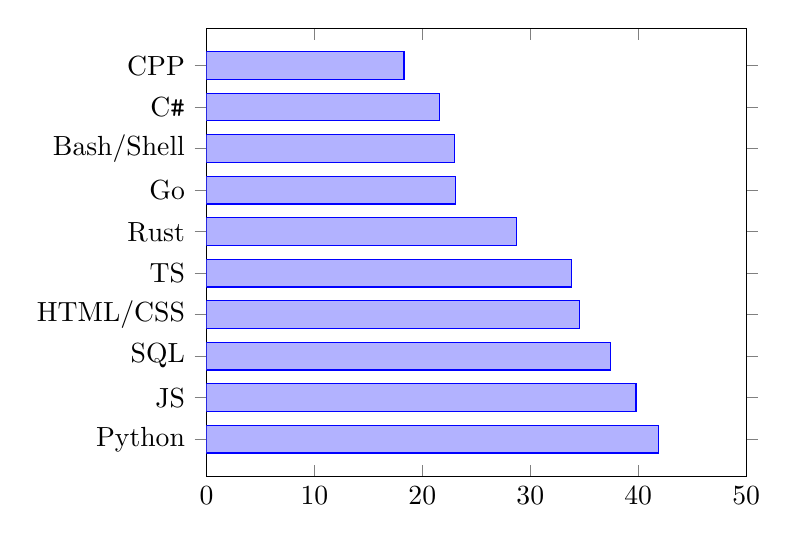
\begin{tikzpicture}
			\begin{axis} [xbar,
					xmin=0,
					xmax=50,
					ytick={0,1,2,3,4,5,6,7,8,9},
					yticklabels={Python, JS, SQL, HTML/CSS, TS, Rust, Go, Bash/Shell, C\texttt{\#}, CPP}]
				\addplot coordinates {
						(41.9,0)
						(39.8,1)
						(37.4,2)
						(34.6,3)
						(33.8,4)
						(28.7,5)
						(23.1,6)
						(23,7)
						(21.6,8)
						(18.3,9)
					};
			\end{axis}
		\end{tikzpicture}
		\caption*{StackOverflow 2024:Most-Desired programming language}
	\end{figure}
\end{frame}

\begin{frame}
	\section{\textcolor{darkmidnightblue}{2. SQL: DDL}}
	Data definition language
	\bigskip

	\begin{quote}
		DDL提供了\alert{定义/修改关系模式}和\alert{删除关系}命令。
	\end{quote}

\end{frame}

\begin{frame}
	\begin{columns}
		\column{0.44\textwidth}<1->
		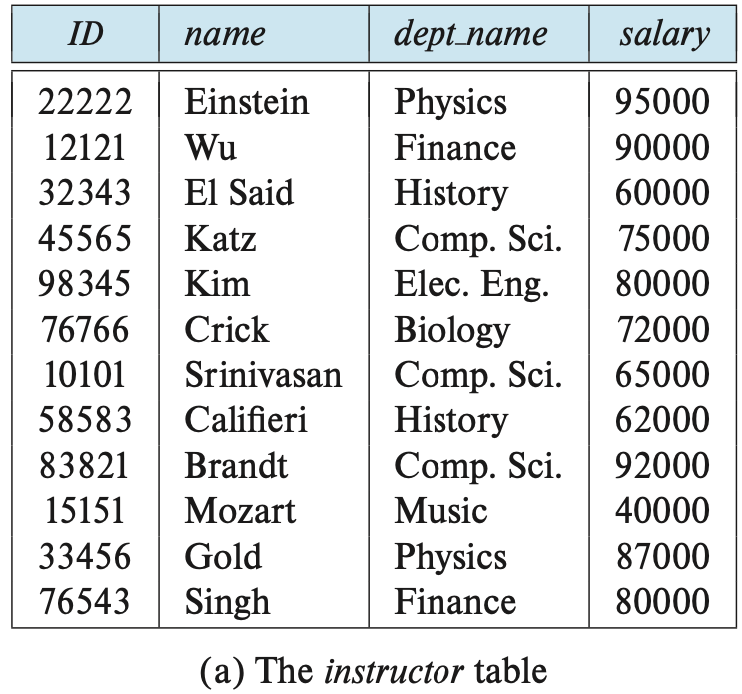
\includegraphics[height=.68\paperheight]{table/instructor}
		\column{0.55\textwidth}<2->
		\begin{enumerate}
			\item \textbf{The schema}
			\item \textbf{The types of values}
			\item \textbf{The integrity constraints}
			\item The set of indices
			\item The security and authorization information
			\item The physical storage Structure
		\end{enumerate}
	\end{columns}



\end{frame}

\begin{frame}
	\frametitle{2.1 基本数据类型(数值)}
	标准 SQL 提供了很多内置的数据类型:
	\begin{itemize}
		\item \texttt{int}:整数类型(与机器相关,等价于 integer)
		\item \texttt{smallint}:小整数整形(int 的子集)
		\item \texttt{numeric(p, d)}:定点数,(最多)有 p 为数字,小数点右边有 d 位 (在 PG 中等价于 \texttt{decimal})
		\item \texttt{float(n)}:精度至少为 n (binary) 位的浮点数
		\item \texttt{real}, \texttt{double precision}:浮点数与双精度浮点数(与机器相关)
	\end{itemize}
	\pause
	{\large \faIcon[regular]{lightbulb}} \texttt{numeric(3, 1)}能表示哪个数?A. 3.14 B. 31.4 C. 314.0
\end{frame}

\begin{frame}
	\begin{table}
		\caption{数值类型}
		\begin{tabular}{lll}
			\toprule
			Name                      & Storage Size & Range                       \\
			\midrule
			\texttt{smallint}         & 2 bytes      & -32768 to +32767            \\
			\texttt{integer}          & 4 bytes      & -2147483648 to +2147483647  \\
			\texttt{real}             & 4 bytes      & 6 decimal digits precision  \\
			\texttt{double precision} & 8 bytes      & 15 decimal digits precision \\
			\bottomrule
		\end{tabular}
	\end{table}

	\begin{itemize}
		\item \texttt{float(1)} 到 \texttt{float(24)}:\texttt{real}
		\item \texttt{float},\texttt{float(25)} 到 \texttt{float(53)}:\texttt{double precision}
	\end{itemize}
\end{frame}

\begin{frame}[fragile]
	\frametitle{2.1 基本数据类型(字符串)}
	\begin{itemize}
		\item \texttt{char(n)}:固定长度的字符串,长度为 n(等价于 \texttt{charater})
		\item \texttt{varchar(n)}:可变长度的字符串,最大长度为 n (等价于 \texttt{character varying})
		\item \texttt{text}:非SQL标准,表示任意长度的字符串
	\end{itemize}
	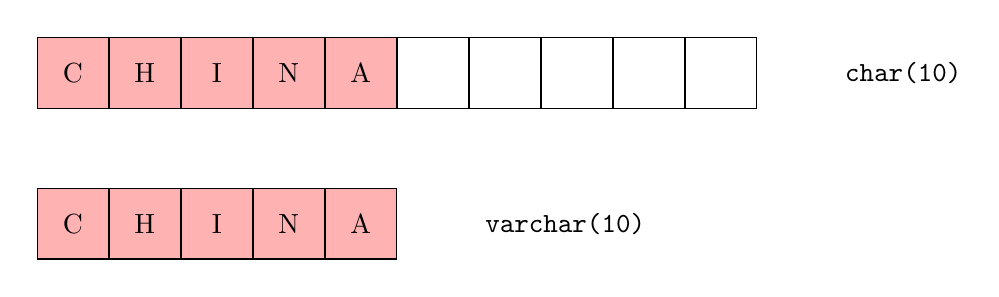
\begin{tikzpicture}[slot/.style={minimum size=0.9cm,rectangle}, data/.style={slot, fill=red!30}]
		\matrix [nodes=draw, row sep=1cm](char) {
			\node[data]{C}; & \node[data]{H}; & \node[data]{I}; & \node[data]{N}; & \node[data]{A};              & \node[slot]{}; & \node[slot]{}; & \node[slot]{}; & \node[slot]{}; & \node[slot](charlast){}; \\

			\node[data]{C}; & \node[data]{H}; & \node[data]{I}; & \node[data]{N}; & \node[data](varcharlast){A};                                                                                                \\
		};
		\node[right=of charlast]{\texttt{char(10)}};
		\node[right=of varcharlast]{\texttt{varchar(10)}};
	\end{tikzpicture}
\end{frame}

\begin{frame}
	\begin{center}
		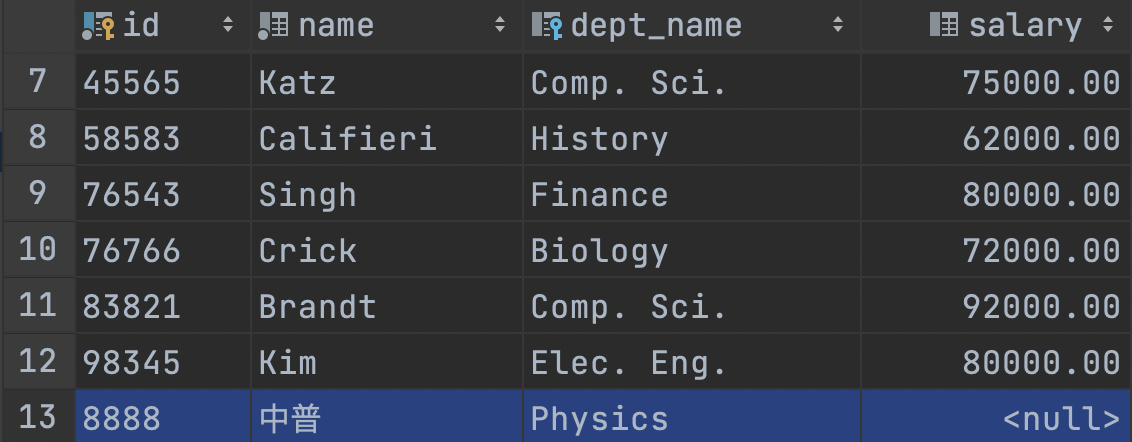
\includegraphics[width=.9\textwidth]{week3/dg-instructor}
	\end{center}
	\texttt{char(n)} 和 \texttt{varchar(n)} 的参数表示\alert{字符串}的长度。所以,\texttt{varchar(2)}能存储可以最多存储 2 个汉字,字节数是 6;也最多存储 2 个字母,字节数为 2。

\end{frame}

\begin{frame}
	\frametitle{2.1 基本数据类型(null)}
	每种数据类型都可能包含一种特殊的值叫做\texttt{null}。它表示一个缺失的值:
	\begin{itemize}
		\item 可能存在但未知(unknown)
		\item 可能不存在
	\end{itemize}
\end{frame}

\begin{frame}[fragile]
	\frametitle{2.2 基本模式定义}
	\begin{minted}[bgcolor=LightGray]{sql}
create table department
    (dept_name  varchar(20),
     building   varchar(15),
     budget     numeric(12, 2),
     primary key (dept_name)); 
    \end{minted}

	\begin{columns}
		\column{.475\textwidth}<1->
		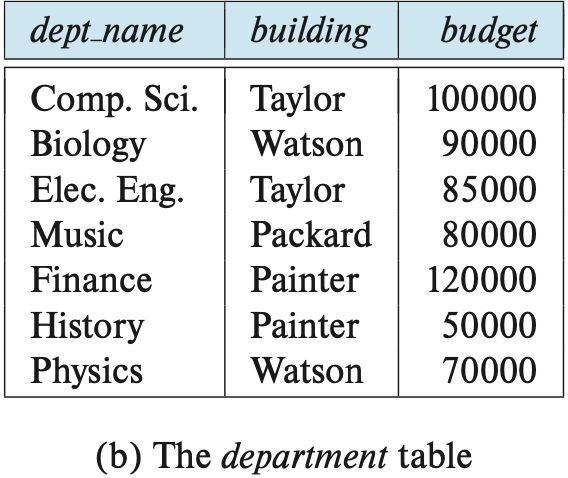
\includegraphics[width=\textwidth,trim={0cm 4cm 0cm 0cm},clip]{table/department}
		\column{.50\textwidth}<2->
		\begin{tikzpicture}
			\node[fill=yellow,blur shadow={shadow xshift=-0.5ex},
				text width=13em,anchor=south west,rounded corners]
			{SQL语句要求使用分号(;)结尾,但是部分数据库不需要。};
		\end{tikzpicture}
	\end{columns}
\end{frame}

\begin{frame}[fragile]
	\begin{minted}[bgcolor=LightGray]{sql}
create table r
    (A1  D1,
     A2  D2,
     ...,
     An  Dn,
     [integrity-constraint 1]
     ...,
     [integrity-constraint k]); 
    \end{minted}
	属性名、数据类型、完整性约束
\end{frame}

\begin{frame}
	\frametitle{码与约束}
	\begin{block}{码}
		码(key):用来区分给定「关系」中的不同「元组」。
	\end{block}
	码的指定也属于被建模的事物在现实世界中的\alert{约束},比如:

	\begin{itemize}
		\item \texttt{primary key}
		\item \texttt{foreign key}
		\item \texttt{not null}
		\item ...
	\end{itemize}

\end{frame}

\begin{frame}[fragile]
	两种风格等价,但不是所有「约束」都有两种写法。

	\begin{minted}[bgcolor=LightGray]{sql}
create table department
    (dept_name  varchar(20),
        building   varchar(15),
        budget     numeric(12, 2),
        primary key (dept_name)); 
    \end{minted}

	\begin{minted}[bgcolor=LightGray]{sql}
create table department
    (dept_name  varchar(20) primary key,
     building   varchar(15),
     budget     numeric(12, 2)); 
        \end{minted}

\end{frame}

\begin{frame}[fragile]
	\begin{minted}[bgcolor=LightGray]{sql}
create table instructor
    (ID     varchar(5), 
     name   varchar(20) not null, 
     dept_name  varchar(20),
     salary     numeric(8,2),
     primary key (ID),
     foreign key (dept_name) references department);
    \end{minted}
	\pause
	部分DBMS(如MySQL)要求外码显式地指出所引用的主码:
	\begin{verbatim}
foreign key (dept_name) references department(dept_name)
\end{verbatim}
\end{frame}

\begin{frame}[fragile]
	\frametitle{2.3 删除}
	\begin{itemize}
		\item 删除表
	\end{itemize}
	\begin{minted}[bgcolor=LightGray]{sql}
drop table r;
\end{minted}

	\begin{itemize}
		\item 清空表数据,但保留表本身
	\end{itemize}
	\begin{minted}[bgcolor=LightGray]{sql}
delete from r;
\end{minted}
\end{frame}

{\setbeamercolor{palette primary}{fg=black, bg=yellow}
\begin{frame}[standout]
	1. 关系名、属性名及关键字(keyword)不分大小写,但一般关键词用大写。

	2. 全部使用英文半角字符。

	3. 具体的语法请查询对应DBMS的文档。
\end{frame}
}

\begin{frame}[fragile]
	\begin{minted}[bgcolor=LightGray]{sql}
/*
Create a table for SWUFE, including:
department name, building name, budget
*/        
CREATE TABLE department
    (dept_name  varchar(20),
     building   varchar(15),
     budget     numeric(12, 2),
     PRIMARY KEY (dept_name)); 

DROP FROM r; -- This is to delete table r
    \end{minted}
\end{frame}
\begin{frame}[fragile]
	\frametitle{思考}
	{\large \faIcon[regular]{lightbulb}} 表名应该使用单数(singular)还是复数(plural)?

	\begin{minted}[bgcolor=LightGray]{sql}
create table product
(
    ...
);

create table products
(
    ...
);
\end{minted}
\end{frame}
\begin{frame}
	\frametitle{练习}

	{\large \faIcon{code}} 设计一个表,用来记录不同城市每日的天气数据,包括城市名、最高气温、最低气温、降雨概率、日期,其中气温记录整数即可。

	提示:日期的类型为 \texttt{date}。
\end{frame}

\begin{frame}[fragile]
	\begin{minted}[bgcolor=LightGray]{sql}
CREATE TABLE weather (
    city          varchar(80),
    temp_lo       int,           -- low temperature
    temp_hi       int,           -- high temperature
    prcp          real,          -- precipitation
    date          date,
    PRIMARY KEY (city, date)
);
    \end{minted}
\end{frame}

\begin{frame}
	\section{\textcolor{darkmidnightblue}{3. SQL: DML}}
	Data manipulation language

	\begin{tikzpicture}
		\node[fill=yellow,blur shadow={shadow xshift=-0.5ex},
			text width=20em,anchor=south west,rounded corners]
		{站着岸上学不会游泳,需要反复上机练习!};
	\end{tikzpicture}
\end{frame}

\begin{frame}[fragile]
	\frametitle{3.1 基本查询结构}
	基本的SQL查询结构包含3个子句: \alert{select},\alert{from},\alert{where}。

	\begin{itemize}
		\item<1-> \(\Pi_{name}(instructor)\)
		      \begin{minted}[bgcolor=LightGray]{sql}
select name from instructor;
    \end{minted}
		\item<2-> 去除重复(duplicate)
		      \begin{minted}[bgcolor=LightGray]{sql}
select distinct dept_name from instructor;
\end{minted}
		\item<3-> \(\Pi_{name, salary/12}(instructor)\)
		      \begin{minted}[bgcolor=LightGray]{sql}
select name, salary / 12 from instructor;
\end{minted}
	\end{itemize}
\end{frame}

\begin{frame}[fragile]
	\alert{where} 子句通过谓词(predicate)选择满足条件的元组;谓词之间可以使用 \texttt{and},\texttt{or},\texttt{not}。

	\[\Pi_{name}(\sigma_{dept\_name=``Physics" \land salary > 70000}(instructor))\]
	\begin{minted}[bgcolor=LightGray]{sql}
select name from instructor 
where dept_name = 'Physics' and salary > 70000;
    \end{minted}
	\pause
	\begin{tikzpicture}
		\node[fill=yellow,blur shadow={shadow xshift=-0.5ex},
			text width=16em,anchor=south west,rounded corners]
		{字符串使用单引号(single quotes)!};
	\end{tikzpicture}
\end{frame}

\begin{frame}[fragile]
	\frametitle{不等于}
	找到非来自 Physics 学院的所有老师的名字

	\begin{minted}[bgcolor=LightGray]{sql}
select name from instructor 
where dept_name != 'Physics';

select name from instructor 
where dept_name <> 'Physics';
\end{minted}

	\begin{tikzpicture}
		\node[fill=yellow,blur shadow={shadow xshift=-0.5ex},
			text width=16em,anchor=south west,rounded corners]
		{\texttt{!=}和\texttt{<>}等价。后者是 SQL 标准。};
	\end{tikzpicture}

\end{frame}

\begin{frame}[fragile]
	\frametitle{between、行构造器}
	\texttt{between} 比较符号,用于简化表达 \texttt{<= and >=}。
	\begin{minted}[bgcolor=LightGray]{sql}    
select name from instructor
where salary between 90000 and 100000;
\end{minted}
	\pause
	行构造器(row constructor ),用于简化多个属性相等。
	\begin{minted}[bgcolor=LightGray]{sql}    
-- Oracle 不支持
select course_id from section
where (semester, year) = ('Spring', 2018);
\end{minted}

\end{frame}

\begin{frame}[fragile]
	\frametitle{3.2 多表查询}
	找出所有老师的名字,这些老师所在的学院名,以及其学院所在楼的名称。
	\begin{itemize}
		\item  \texttt{instructor(ID, name, dept\_name, salary)}
		\item \texttt{department(dept\_name, building, budget)}
	\end{itemize}
	\[\Pi_{name, instructor.dept\_name, building}(instructor \Join department)\]

	\begin{minted}[bgcolor=LightGray]{sql} 
select name, instructor.dept_name, building 
from instructor, department
where instructor.dept_name = department.dept_name;
\end{minted}

\end{frame}

\begin{frame}[fragile]
	\begin{minted}[bgcolor=LightGray]{sql} 
select A1, A2, ..., An
from r1, r2, ..., rm
where P;
    \end{minted}
	更易于理解的方式是:先 \texttt{from},再 \texttt{where},最后 \texttt{select}。
\end{frame}

\begin{frame}[fragile]
	\frametitle{练习}
	{\large \faIcon{code}} 找出所有计算机学院的老师名字及其讲授课程的课程号。

	\begin{itemize}
		\item \texttt{instructor(ID, name, dept\_name, salary)}
		\item \texttt{teaches(ID, course\_id, sec\_id, semester, year)}
	\end{itemize}
	\pause
	\begin{minted}[bgcolor=LightGray]{sql} 
select name, course_id
from instructor, teaches
where instructor.ID = teaches.ID 
      and instructor.dept_name = '计算机';
    \end{minted}
\end{frame}
\begin{frame}
	\section{\textcolor{darkmidnightblue}{4. 附加SQL操作}}
	更名、排序等
\end{frame}
\begin{frame}
	\frametitle{4.1 更名 (rename)}
	{\large \[\rho_x(E)\]}
	将表达式\texttt{E}更名为\texttt{x},如:\[\rho_{physicist}(\sigma_{dept\_name=``Physics"}(instructor))\]

	还可以进一步对属性进行更名,如:\[\rho_{instructor(ID, name, dept, year\_salary)}(instructor)\]

\end{frame}

\begin{frame}[fragile]
	SQL更名使用 \texttt{as} 命令,可以出现在 \texttt{from} 和 \texttt{select} 子句。用法是:
	\begin{verbatim}
old_name as new_name    
\end{verbatim}

	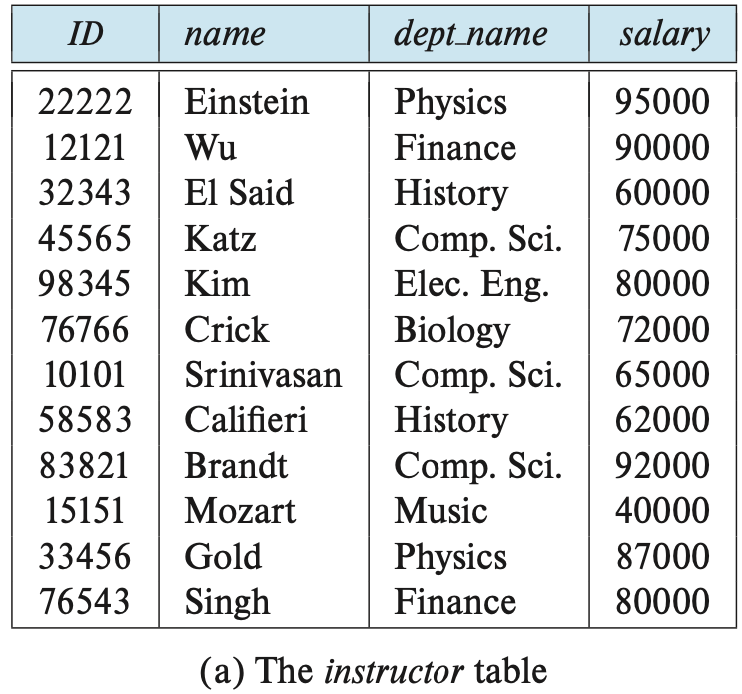
\includegraphics[width=.6\textwidth,trim={0cm 8.5cm 0cm 0cm},clip]{table/instructor}

	\begin{minted}[bgcolor=LightGray]{sql} 
select name as teacher from instructor;
\end{minted}

\end{frame}

\begin{frame}[fragile]

	\begin{minted}[bgcolor=LightGray]{sql} 
select name, course_id
from instructor, teaches
where instructor.ID = teaches.ID;   

select name, course_id
from instructor as T, teaches as S
where T.ID = S.ID ;
    \end{minted}

\end{frame}

\begin{frame}[fragile]
	\frametitle{4.2 * (asterisk)}
	\texttt{*}表示“所有的属性”。

	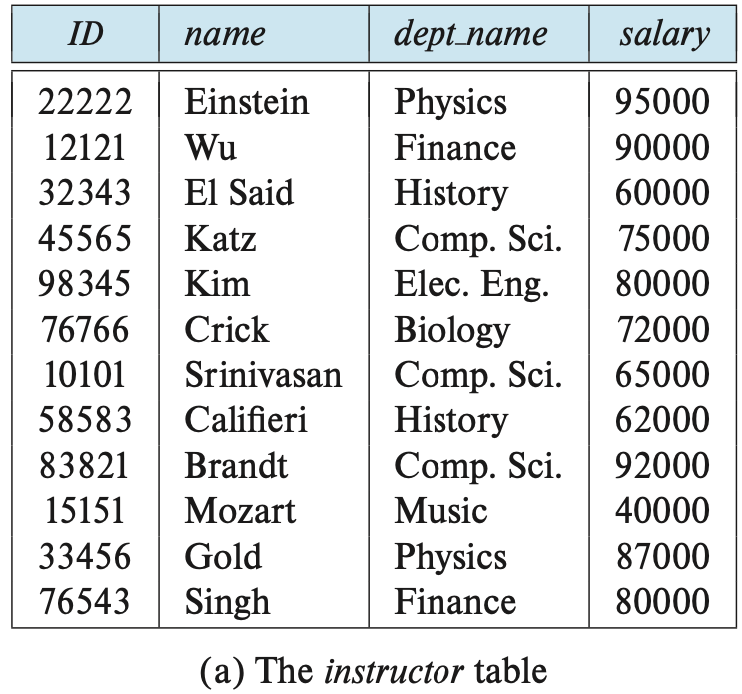
\includegraphics[width=.6\textwidth,trim={0cm 8.5cm 0cm 0cm},clip]{table/instructor}

	\begin{minted}[bgcolor=LightGray]{sql} 
select * from instructor;
\end{minted}

	\begin{tikzpicture}
		\node[fill=yellow,blur shadow={shadow xshift=-0.5ex},
			text width=23em,anchor=south west,rounded corners]
		{在测试时很方便,但不建议在生产环境下使用。};
	\end{tikzpicture}

\end{frame}

\begin{frame}[fragile]
	\frametitle{4.3 排序}
	使用 \texttt{order by} 子句,默认是升序(ascending order)。为了指定排序方式,可以使用 \texttt{desc} (descending,降序)和 \texttt{asc} (升序)。

	\begin{minted}[bgcolor=LightGray]{sql} 
select *
from instructor
order by salary desc, name asc;        
    \end{minted}

	\pause {\large \faIcon[regular]{lightbulb}} \textbf{思考}:\alert{\texttt{order by A, B desc}} 是如何排序的?
\end{frame}

\begin{frame}
	\section{\textcolor{darkmidnightblue}{总结}}
	\begin{enumerate}
		\item 基本类型(数、字符串)
		\item 定义关系(\texttt{create table})
		\item 查询关系(\texttt{select}, \texttt{from}, \texttt{where})
		\item 更名运算(\texttt{as})、排序子句(\texttt{order by})
	\end{enumerate}
\end{frame}
\begin{frame}
	\frametitle{Homework 2}
	\href{https://github.com/ChenZhongPu/db-swufe/tree/master/03_basic_sql}{03. Basic SQL}

	\noindent\rule{\textwidth}{1pt}

	确保安装PG和DataGrip软件,并下载GitHub上的SQL代码,为下周的实验课做好准备。

\end{frame}
\end{document}
